\section{Implementing a Graphical User Interface (GUI) Framework, and the Power of Lenses}
\label{sec:gui}

Gloss provided an interim layer to abstract away the complexities of OpenGL and impure drawing code, but as it turned out further abstractions on top of this were desirable. Gloss provides no ``widgets'' (buttons, scroll bars, etc), nor does it facilitate separable concerns for event handling.

\begin{marginfigure}
	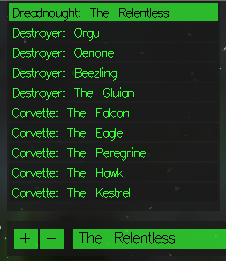
\includegraphics{res/sheen/fleetbuilder1.png}
	\caption[Fleet builder UI built using Sheen]{Part of the fleet builder UI built using.}
	\label{fig:openglbasicout}
\end{marginfigure}

Some time was spent in developing a framework on top of Gloss to enable easier construction of graphical interfaces, which has been glibly titled \emph{Sheen}\index{Sheen}. Provided by Sheen is a mechanism for event handling, recursively nested views, and various pre-built widgets such as labels, buttons, and text boxes. The best approach to the design of Sheen was not obvious, and its structure, and use of \emph{lenses} (see below) is considered to be quite novel and a demonstration of good Haskell style. This section considers various aspects of the Sheen design, but first it is worth examining lenses as significant use of them are made in the framework.

\subsection{On Lenses}

A lens is the functional equivalent of a setter and a getter at the same time. One way of thinking of a lens is it having the type

\functions(view, get, set, lens)
>data Lens a b = {get :: a -> b, set :: b -> a -> a}

Normally lenses are not actually implemented this way, but in such a way to be isomorphic to this. The most popular implementation of lenses is currently in the \emph{lens} package by Edward Kmett,\sidenote{Edward A. Kmett, Copyright 2012-2013 \url{https://github.com/ekmett/lens/}.} which uses a generalised form of a so called van Laarhoven lenses. A van Laarhoven lens has type

>type SimpleLens a b = forall f. Functor f => (b -> f b) -> a -> f a

and the generalised notion of a lens family has type

>type Lens a b c d = forall f. Functor f => (c -> f d) -> a -> f b

The advantage of this definition of lenses is that they can be composed normally as functions using "(.)" and "id" from the Haskell prelude. This, and the large number of combinators provided in the \emph{lens} package, is partly what makes lenses so vastly useful. For a full technical explanation of this implementation of lenses see \url{comonad.com/reader/2012/mirrored-lenses}; here the way they are used is all that need be considered.

\functions(makeLenses, makeClassy, _bar, _baz, bar, baz, sndLens)
There are two ways of creating lenses. First is to use the "lens" function to build the lens from a getting and setting function directly, for example

>sndLens = lens snd (\(a,_) b -> (a,b))

This leads to a lot of boilerplate however. The alternative is to use the template Haskell routines provided in the library, "makeLenses" or "makeClassy". These do require Template Haskell (and hence GHC) but are very useful indeed. In the expression

>data Foo a = Foo
>  {  _bar :: a
>  ,  _baz :: [a]
>  }
>makeLenses ''Foo

the last line will create two addition functions

>bar :: Functor f => (a -> f a) -> Foo a -> f (Foo a)
>baz :: Functor f => ([a] -> f [a]) -> Foo a -> f (Foo a)

Or the same thing expressed in the "Lens" type synonym: 

>bar :: Simple Lens (Foo a) a
>baz :: Simple Lens (Foo a) [a]

This demonstrates how easy it is create lenses with Template Haskell, but why is it worth doing? Lenses are invaluable for providing good interfaces between modules and hence separation of concerns. For example, say one module contains the overall state of an application, and another module is responsible for logic based on only a part of that state. By making the functions in this latter module depend, rather than the specific data type that contains the application state, but rather any type "a" and lenses from "a" onto the parts of the data that module is responsible for, the modules remain nicely separated. This technique is leveraged extensively when using Sheen.

\subsection{Recursive Views}

In the prototype projects written with Gloss, widgets were modelled quite simply as having an area of the screen that would trigger actions when an event fell within the bounds. This was unsatisfactory  for a number of reasons. First, and especially as Gloss has no support for clipping,\sidenote{Clipping is masking out parts of an image so that only one area of the screen can be drawn to.} was care that had to be taken that the picture of the widget ended up in the same place as its target area. And also there is the problem that as the layouts become more complicated, connascence between all the different widgets builds up. If one wanted to move an entire sidebar, for example, everything within it would require its position updating. Hardly ideal.

Sheen was first created to solve this sole issue, by supporting the concept of a recursive structure. The definition of "View" in the latest sheen code is

\vspace{-0.5em}
\begin{listing}{list:sheenview}{Definition of a \emph{View} in Sheen.}{Definition of a \scalenote{"View"} in Sheen. Some fields non-essential to the discussion are not shown.}{}
\end{listing}\vspace{-1.5em}

\functions(_viewSubviews, _viewFrame, _viewZIndex, _viewBackground, _viewDepict, _viewDepictMode, _viewSubviewMode, _viewEventHandler)
\begin{haskell}

>data View a = View
>  {  _viewSubviews     :: [View a]
>  ,  _viewFrame        :: Extent
>  ,  _viewZIndex       :: Int
>  ,  _viewBackground   :: Maybe Color
>  ,  _viewDepict       :: Maybe Picture
>  ,  _viewEventHandler :: Maybe (UIEvent -> a)
>  }

\end{haskell}
\noindent 
Note that the subviews field makes this a recursive structure. In order to support concepts like focus of text boxes and other stateful behaviour, the view system needs somewhere to store state. For this reason the top level of view hierarchy is required to be a member of the "ViewController" class, as shown below.

\vspace{-0.5em}
\begin{listing}{list:sheenview}{\emph{ViewController} class.}{\scalenote{"ViewController"} class.}{}
\end{listing}\vspace{-1.5em}

\functions(globals, getView)
\begin{haskell}

>class ViewController a where
>  globals :: Simple Lens a (ViewGlobals a)
>  getView :: a -> View a
>  updateTime :: Float -> a -> a
>  updateTime _ = id

\end{haskell}
\noindent 

